\documentclass{article}

\usepackage[margin=1in]{geometry} 
\usepackage{authblk}
\usepackage{amsmath}
\usepackage{graphicx}
\usepackage{float}
\usepackage{hyperref}

\hypersetup{
    colorlinks=true,
    linkcolor=blue,
    filecolor=magenta,      
    urlcolor=blue,
    pdftitle={Effects of anthropogenic aerosol emissions},
}

%\usepackage[backend=biber]{biblatex}

%\addbibresource{ref.bib}

\author{Abhaygnanaskandan S}
\title{Effects of anthropogenic aerosol emissions}
\date{\vspace{-5ex}}

\begin{document}
\maketitle

%\tableofcontents 
\vspace{2em}

\section{Introduction}
\indent Humans emit a lot of pollutants into the atmosphere that can change the albedo of Earth. These pollutants include: black carbon(soot), primary organic matter, $SO_{4}$, $SO_{2}$, secondary organic aerosol gas.\\

\indent In this project, I have reduced all anthropogenic emissions mentioned above that affect albedo by 50\% and 100\% to study the effects of these emissions on clouds and Indian summer monsoon.\\

\section{Case structure}
 Model: CESM2.0.0\\
 \indent \textbf{Ref:} \url{https://docs.cesm.ucar.edu/models/cesm2/config/2.0.0/}\\
 
 Grid: f09\_f09\_mg17\\
 \indent resolution: $0.9^\circ \times 1.25^\circ$\\
 
 Compset: F2000climo\\
 \indent Present day data year: 2000\\ 
 \indent Prescribed: sea ice, ocean, land ice\\
 \indent Components: Atmosphere: CAM, Land: CLM, River runoff: MOSART\\

 Spin-up period: 12 years\\
 Analysis period: 3 years\\

 \indent For the branch cases, all the input nc files with anthropogenic emissions were modified according to the specific branch case.\\

\section{Model spin-up}

\indent Before running our experiment of reducing aerosols. we have to let our model ``spin-up" from the set initial condition so that energy, temperatures don't fluctuate much.\\
\indent The following are the plots to check model spin-up.\\
\begin{figure}[H]
    \centering
    
\includegraphics[width=\textwidth]{spinup_sfc_temp.png}
    \caption{Surface temperature during spinup}
    \label{fig:spinup_sfc_temp}
\end{figure}
\indent The oscillation of temperature might be due to the elliptical orbit of earth(Cannot be seasonal variation as it is global average temperature and it is always summer in one of the hemispheres).

\begin{figure}[H]
    \centering
    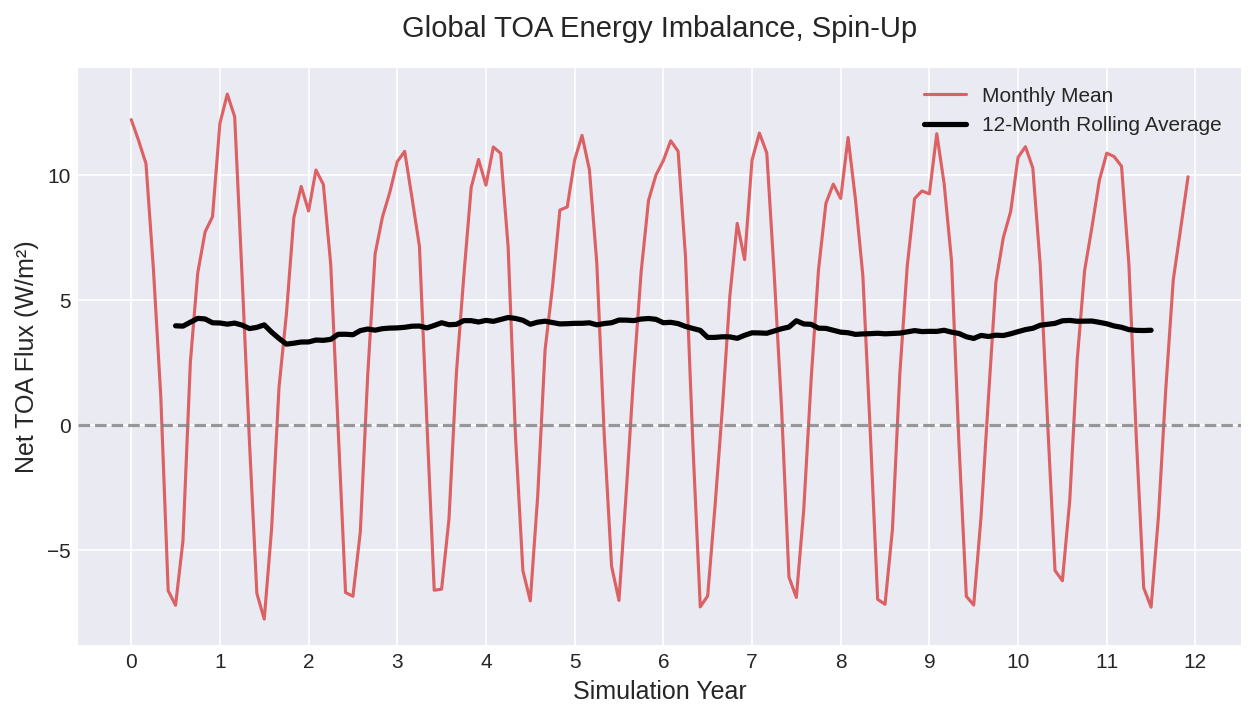
\includegraphics[width=\textwidth]{spinup_toa_e.png}
    \caption{TOA energy imbalance during spinup}
    \label{fig:spinup_toa_e}
\end{figure}
\indent Oscillation of TOA radiation flux is due to same reason mentioned previously. The average is not 0 as the oceans have a constant temperature in this model, therefore they act as an energy source.\\

\indent Since the ocean is prescribed in F2000climo, that is, it is just an atmospheric model, the spin-up period is not that long.\\

\indent Since the land component is the slowest evolving component of this model, we have to check for its spin-up.\\
\begin{figure}[H]
    \centering
    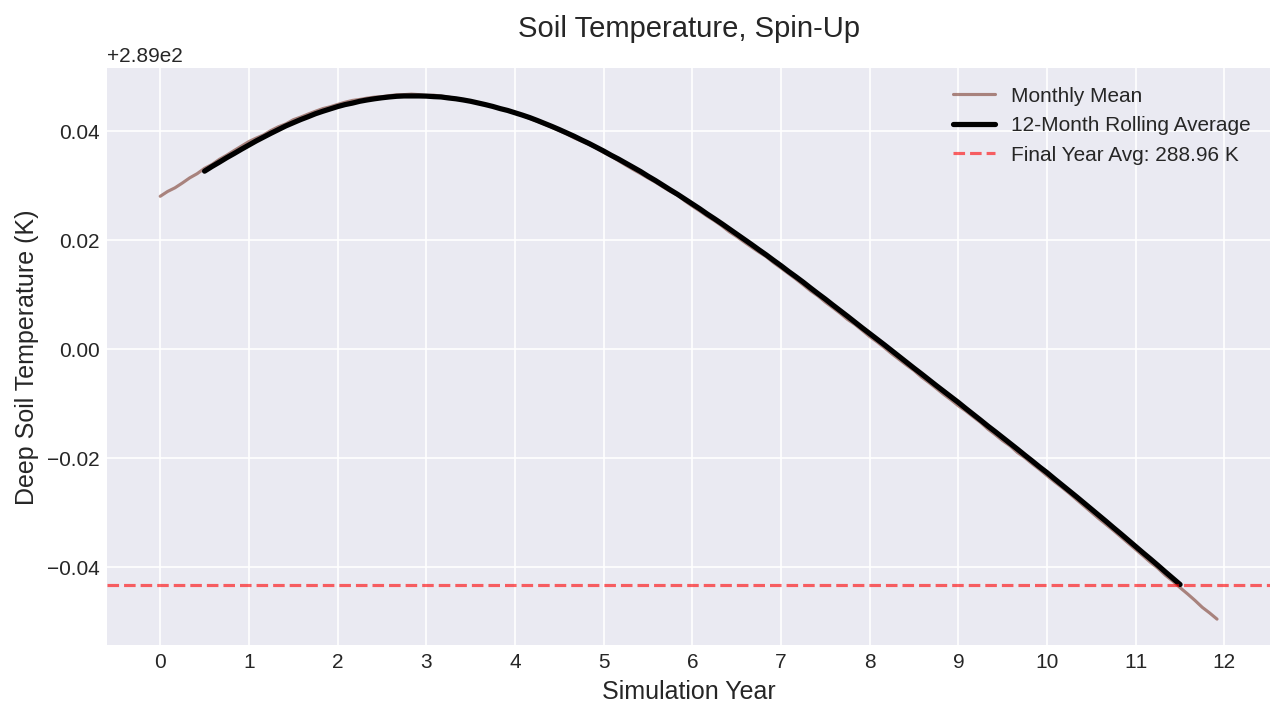
\includegraphics[width=\textwidth]{spinup_deep_soil.png}
    \caption{Soil temperature during spinup}
    \label{fig:spinup_soil}
\end{figure}
\indent The above plot shows temperature difference from 289K. Since the fluctuation is small, we can say that the model has spun up.\\

\section{Results and Inferences}
\indent All anomalies were calculated by subtracting the control case data from the data of the specific case.\\

\subsection{Validation of aerosol reduction}
\indent First, we have to check if the reduction of aerosols had worked or not. We can confirm this by plotting the optical depth.\\
\begin{figure}[H]
    \centering
    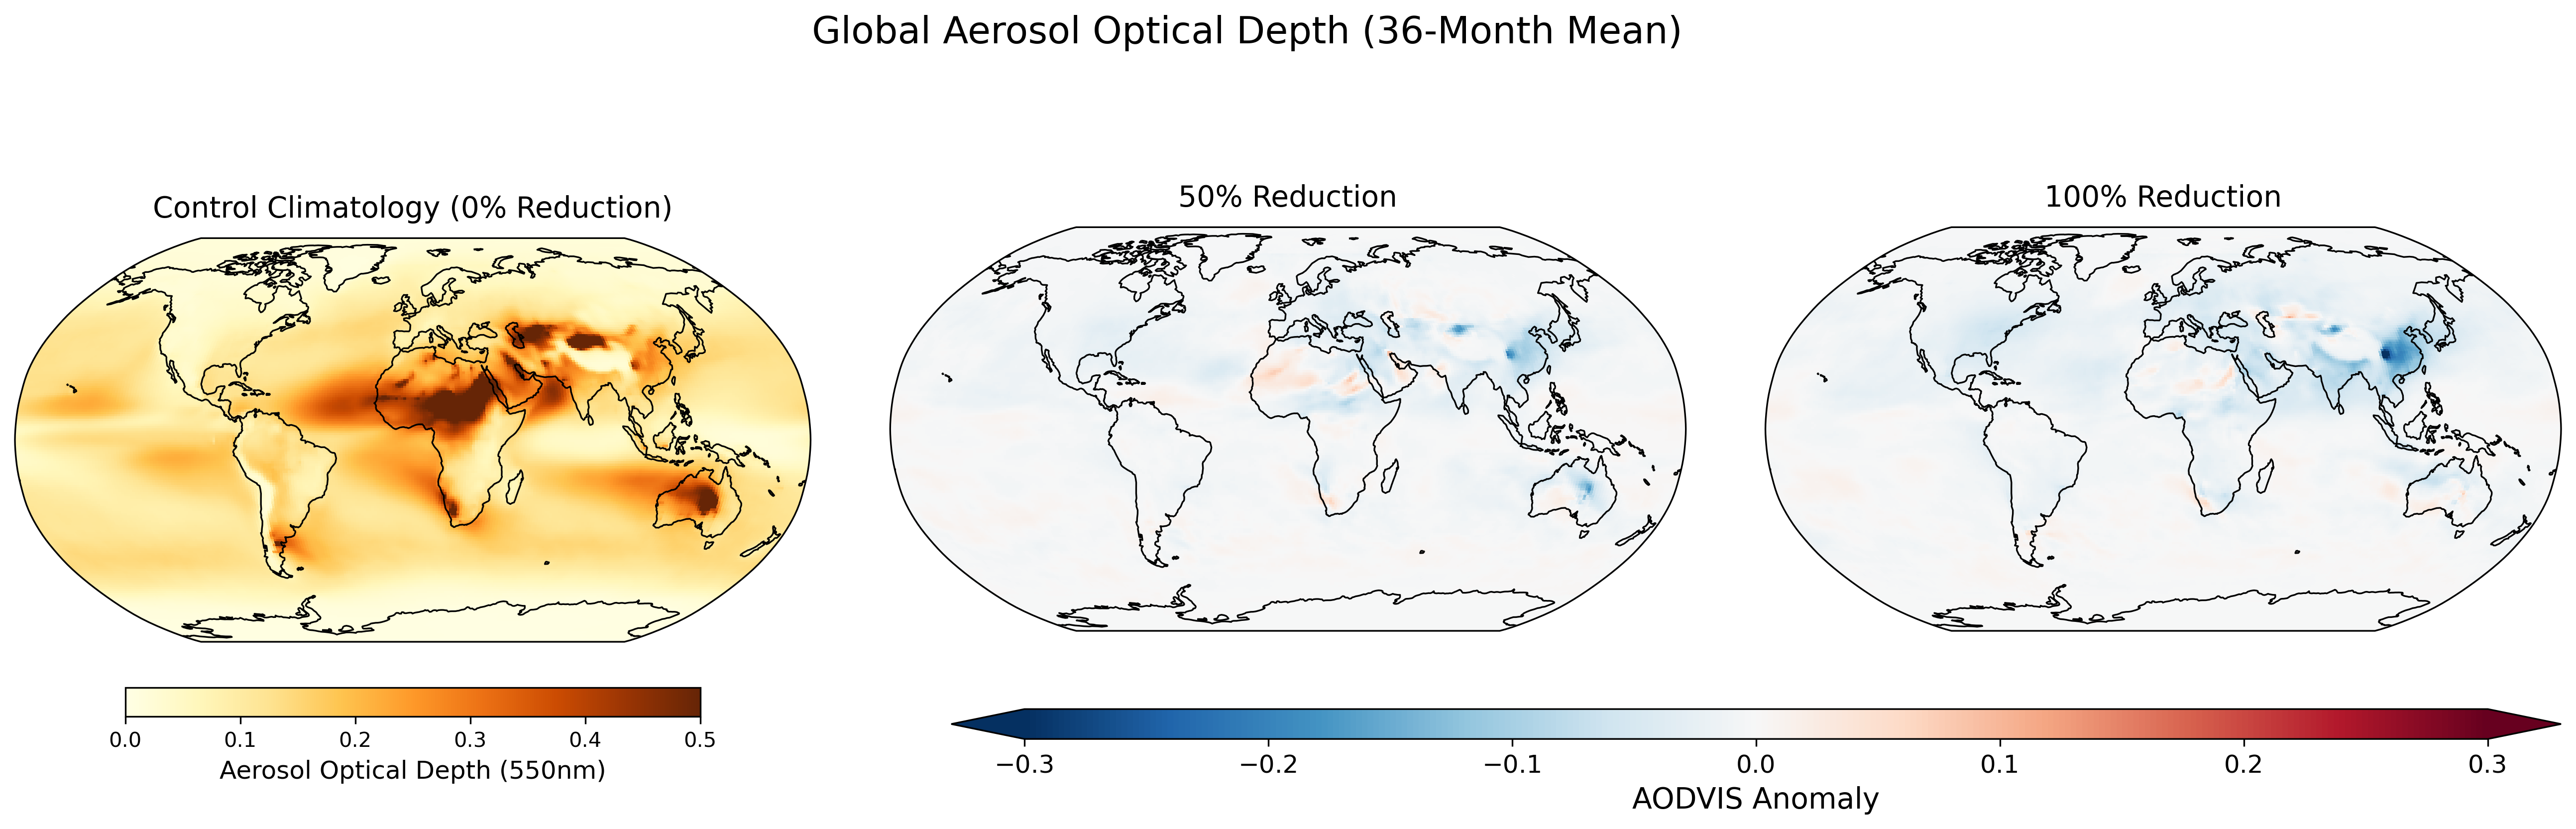
\includegraphics[width=\textwidth]{opt_depth.png}
    \caption{Optical depth}
    \label{fig:optical_depth}
\end{figure}

\indent The following is the plot of incoming shortwave radiation at the surface.\\
\begin{figure}[H]
    \centering
    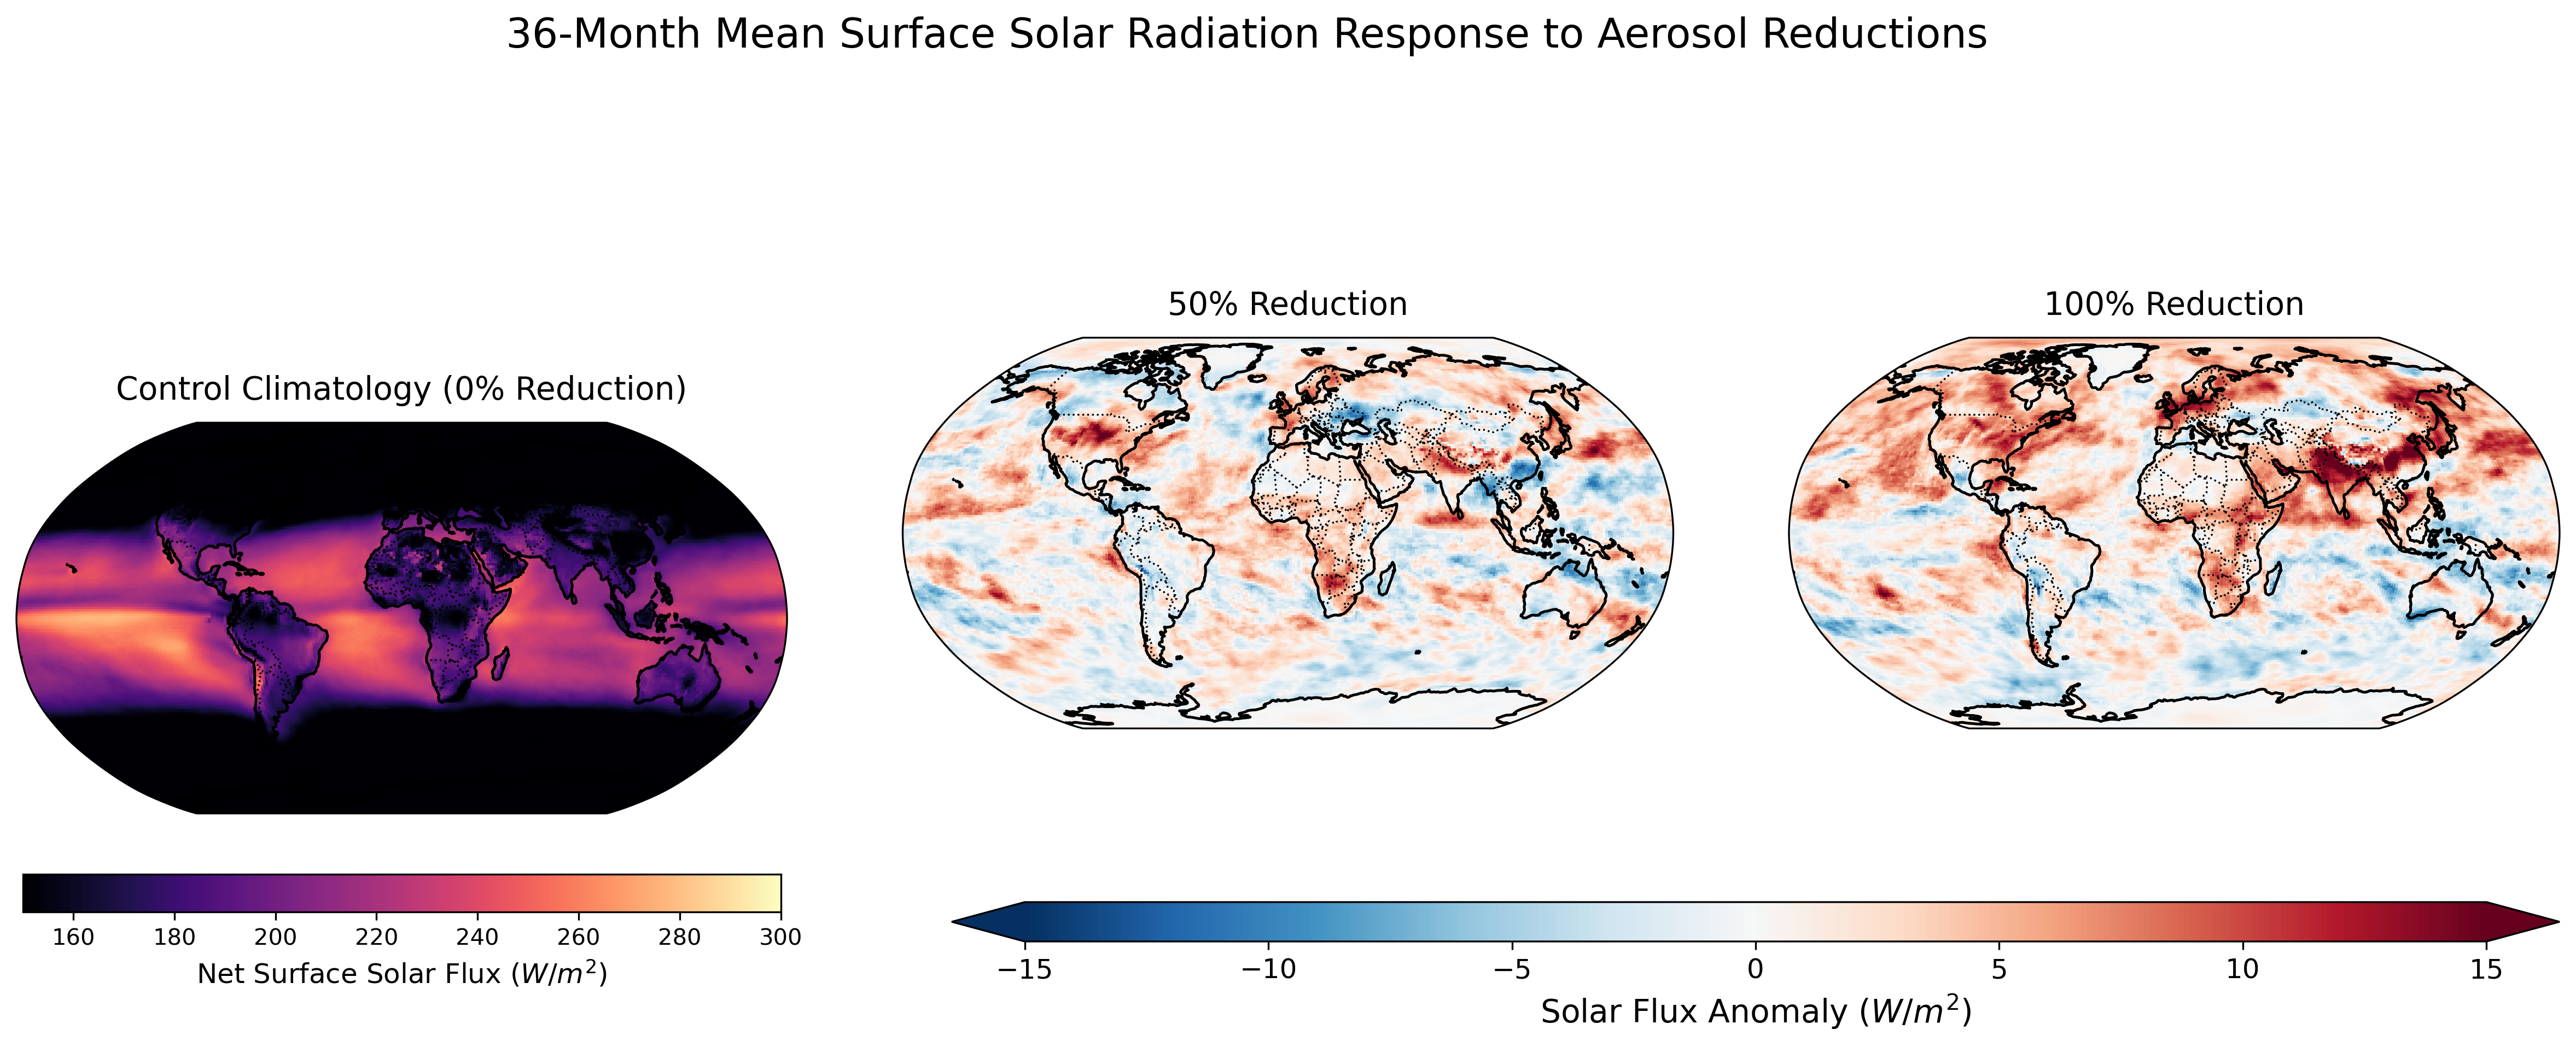
\includegraphics[width=\textwidth]{shortwave.png}
    \caption{incoming shortwave radiation at surface}
    \label{fig:sfc_shortwave}
\end{figure}
\indent Since the aerosol concentration has decreased, the net albedo has decreased, so we see an increase in the incoming shortwave radiation at the surface level. We can also see that the anomalies are highest in industrial regions that tend to emit a lot of aerosols.\\

\indent The following is the plot of energy imbalance anomalies at the top of the atmosphere.\\
\begin{figure}[H]
    \centering
    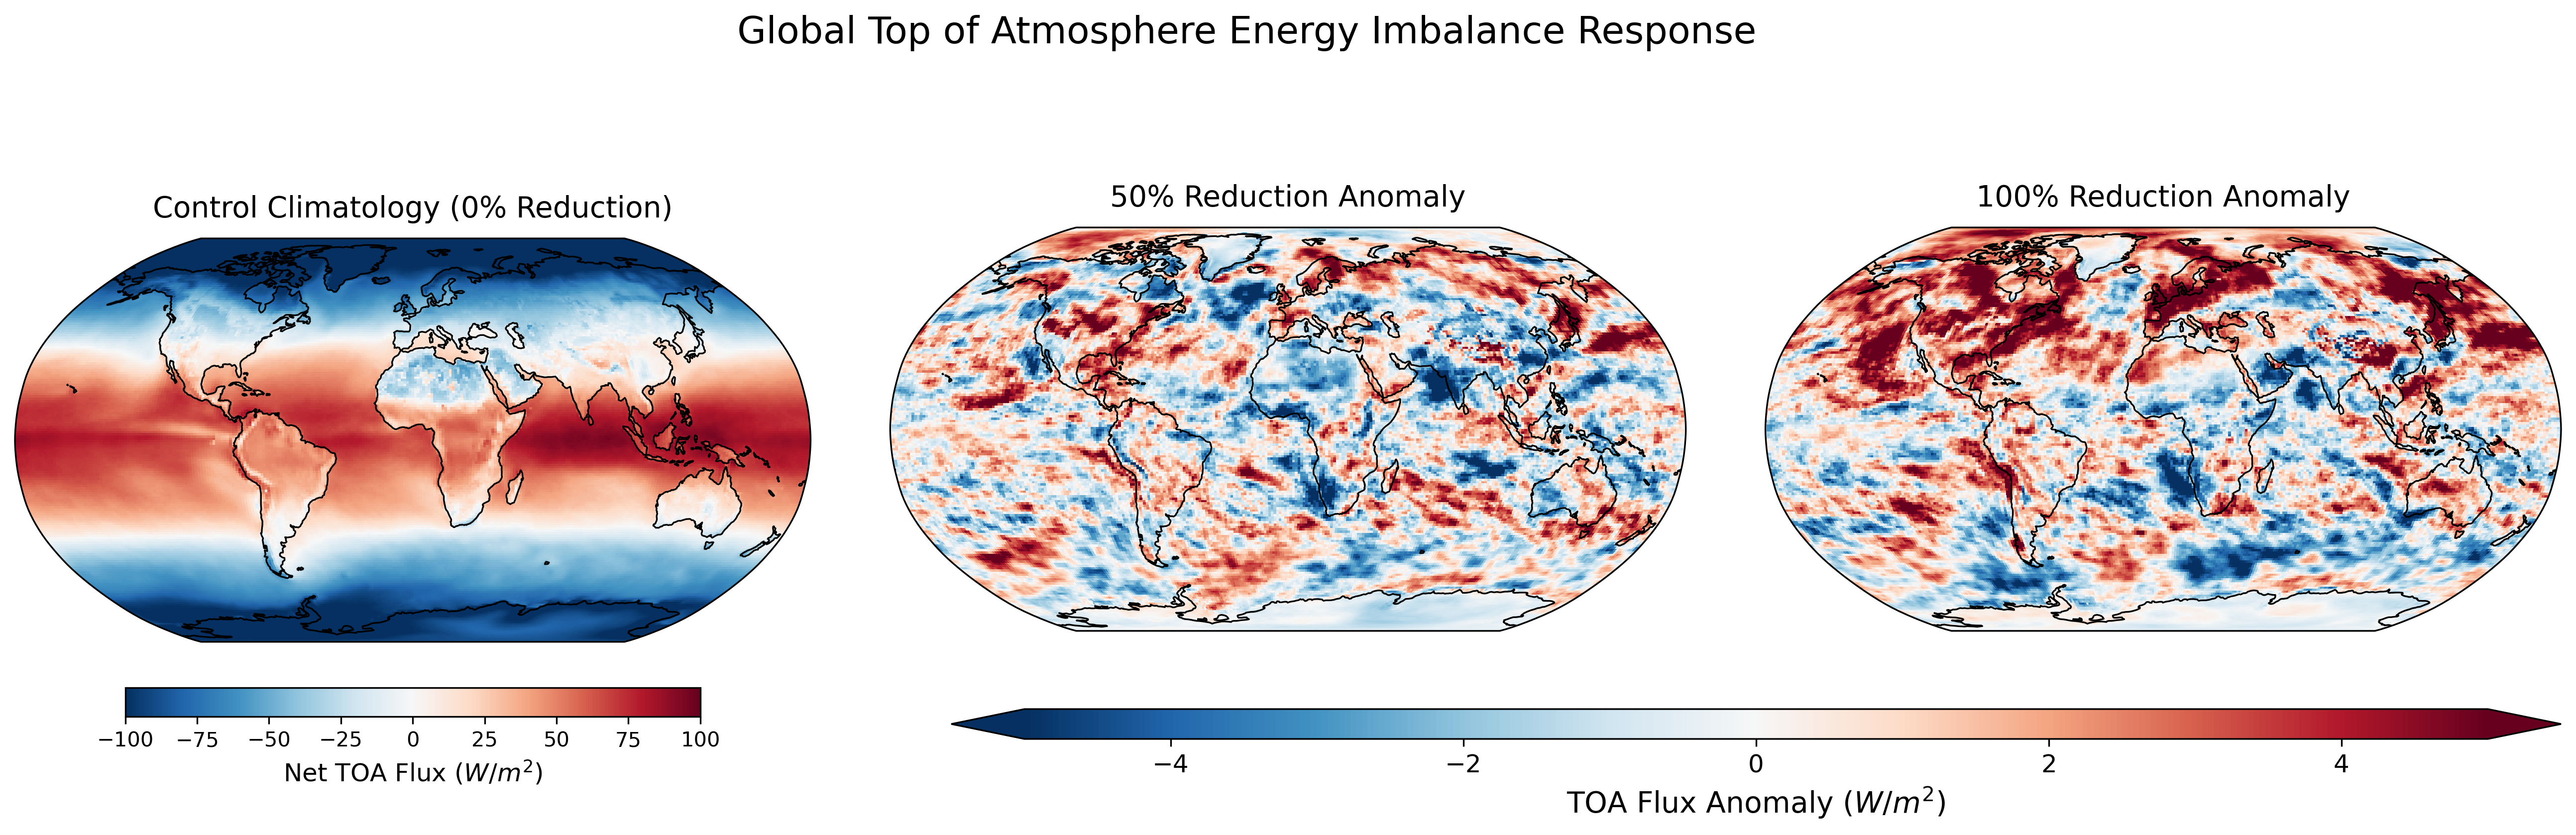
\includegraphics[width=\textwidth]{toa_e.png}
    \caption{Energy anomaly at the top of the atmosphere}
    \label{fig:toa_e}
\end{figure}

\indent Now that we have confirmed that the aerosol has reduced in the model, we can study the effect of aerosol emissions on various things. I have chosen to study its effect on clouds and Indian summer monsoon.\\

\subsection{Effect on clouds}

\indent Some of the aerosols that we emit act as nucleation sites for clouds. So, when emission is decreased we should see a drop in the number of condensed water droplets.\\
\begin{figure}[H]
    \centering
    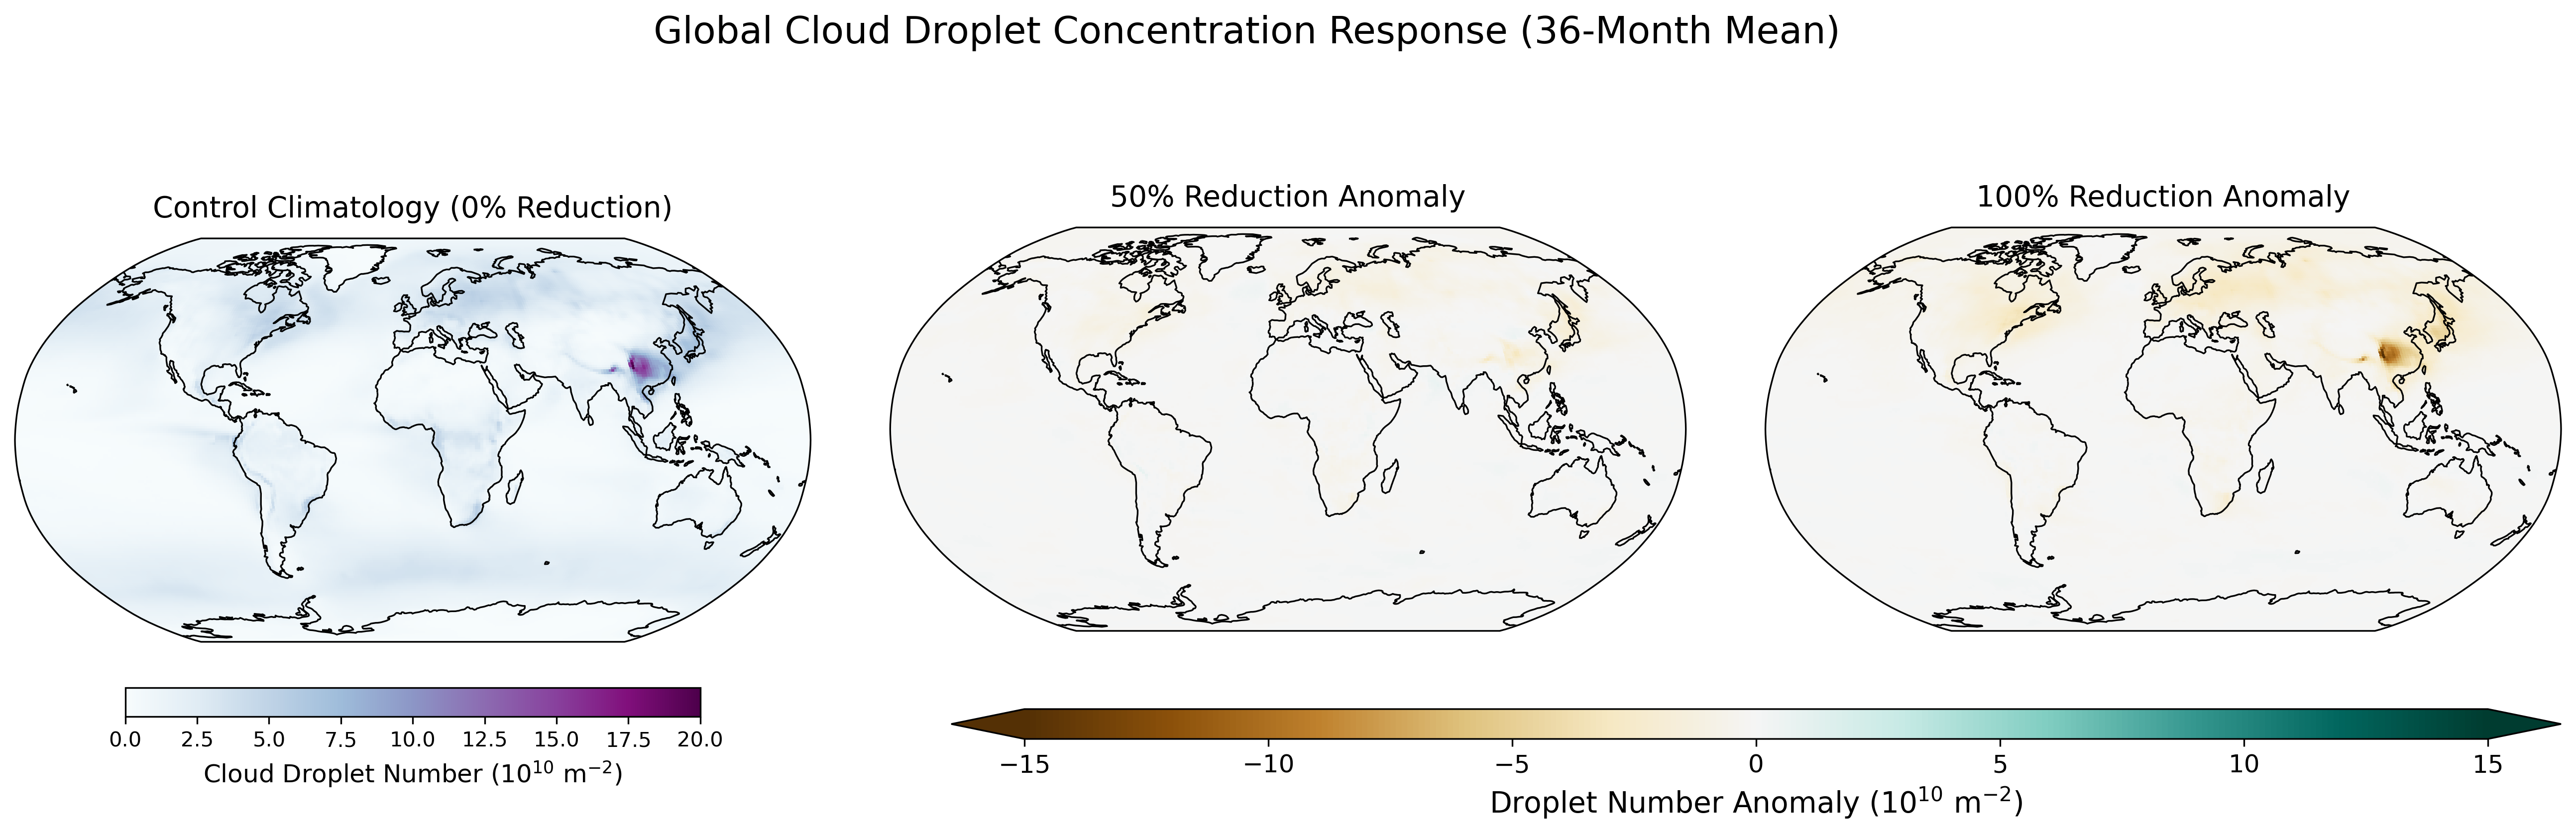
\includegraphics[width=\textwidth]{num_cloud.png}
    \caption{Number of cloud nucleation site}
    \label{fig:num_cloud}
\end{figure}
\indent We see a reduction in the number of cloud droplets in the Chinese region where there is a lot of aerosol emissions.\\

\indent Low number of water droplets would imply larger droplet size, which is more immune to getting evapourated when a dry parcel of air enters the cloud. It also means lack of nucleation sites for the drops to form initially. We can find the net effect by plotting the total cloud cover anomaly.
\begin{figure}[H]
    \centering
    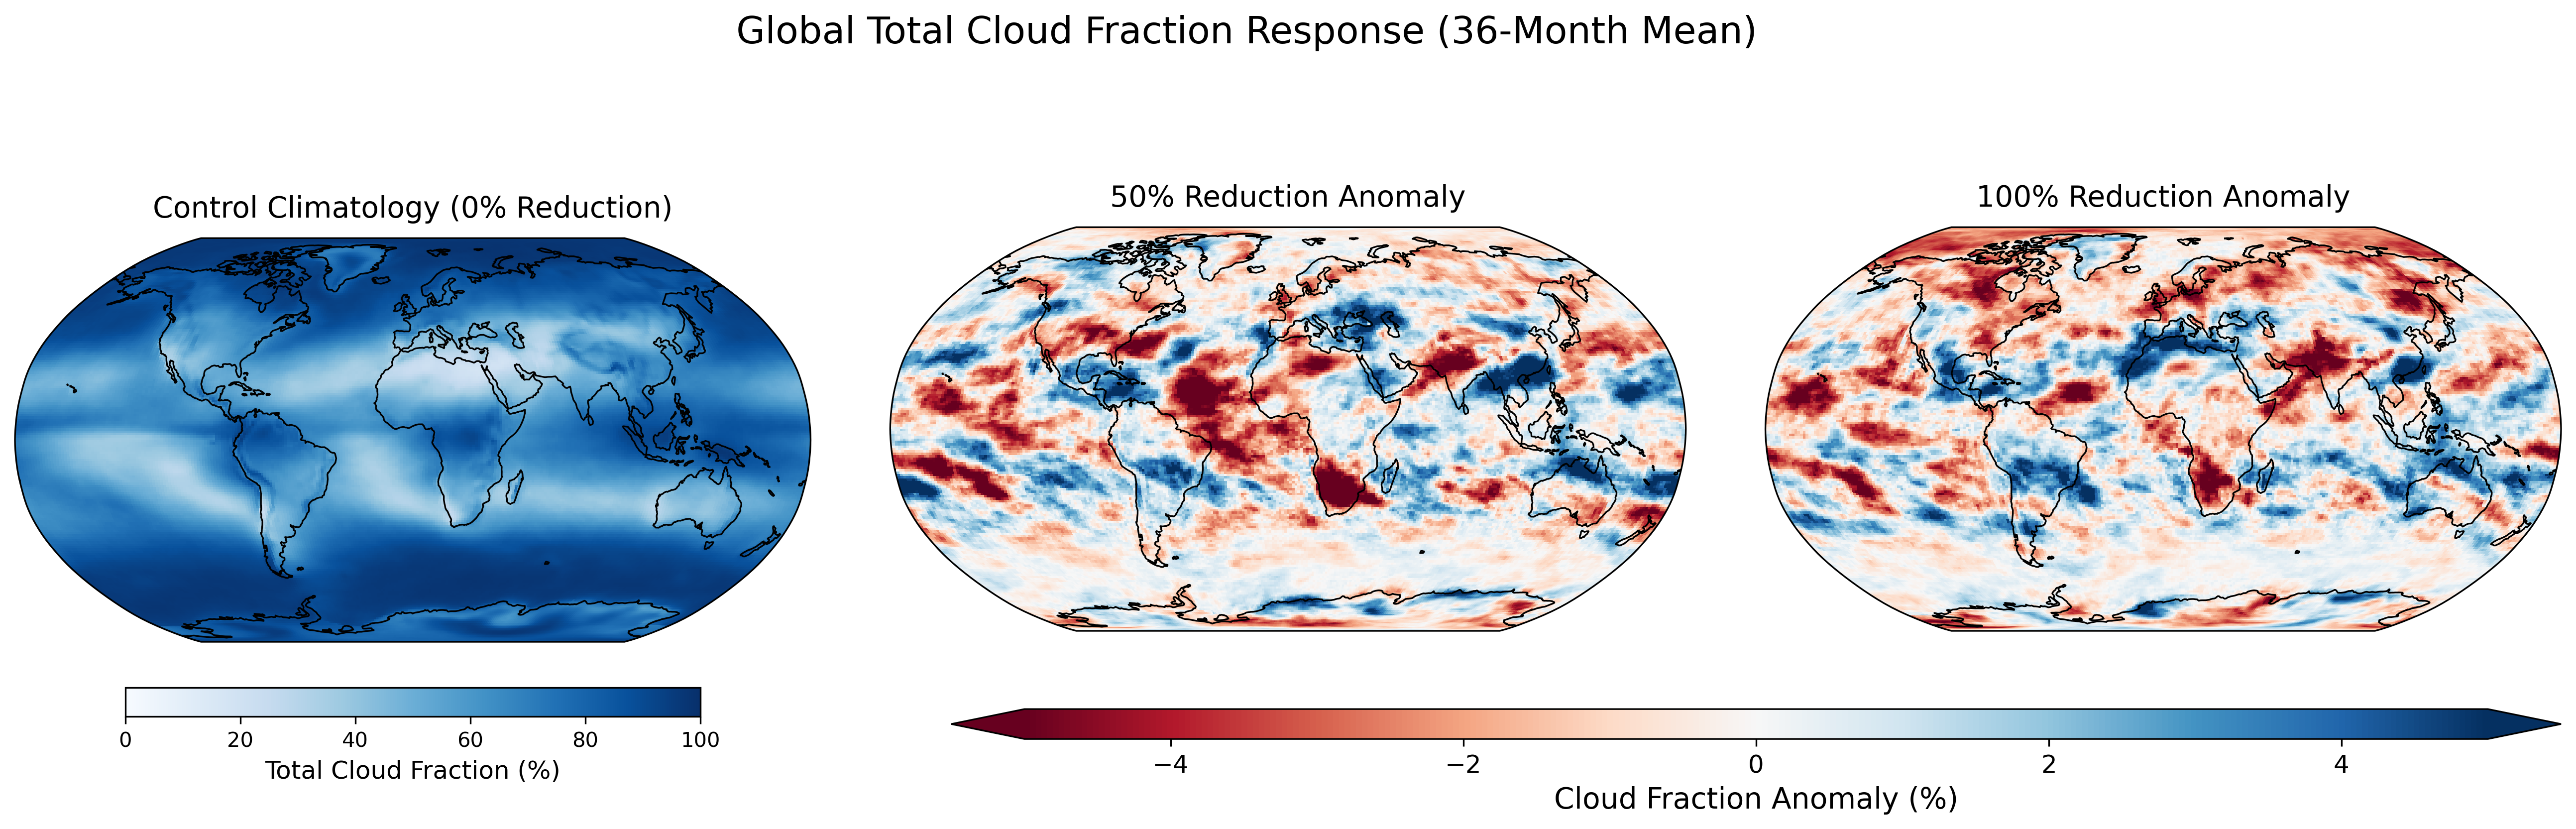
\includegraphics[width=\textwidth]{total_cloud.png}
    \caption{Total cloud cover}
    \label{fig:total_cloud_cover}
\end{figure}
\indent The above plot shows how the cloud cover would change in each region if aerosol emissions were reduced.\\
\subsection{Effect on Indian summer monsoon}

\indent The following is the surface temperature anomaly plot of the Indian region.\\
\begin{figure}[H]
    \centering
    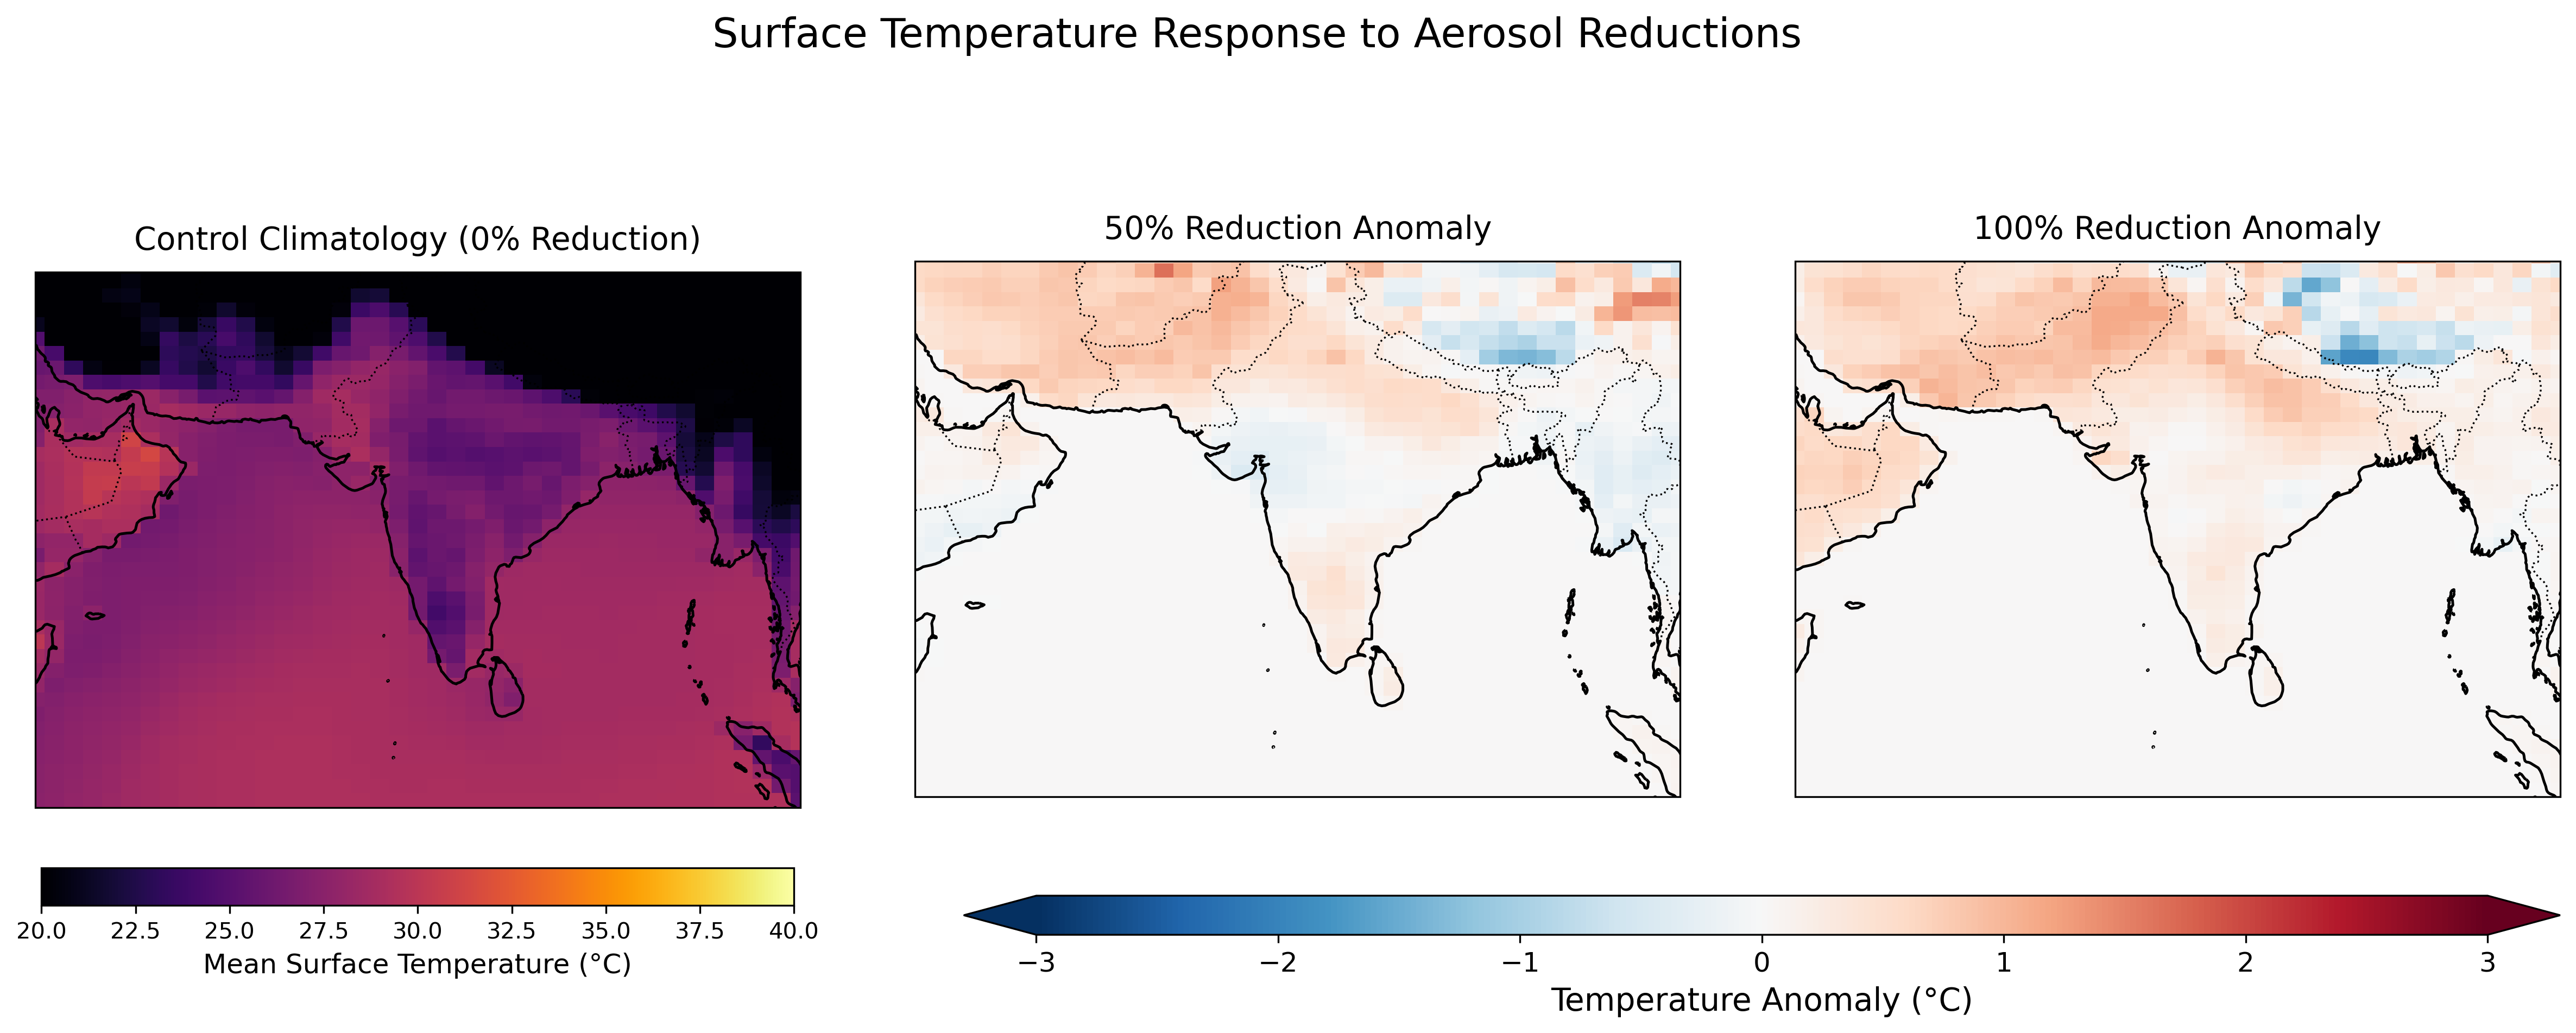
\includegraphics[width=\textwidth]{temp.png}
    \caption{Surface temperature}
    \label{fig:sfc_temp}
\end{figure}
\indent We see that due to reduction of aerosol emissions, the land temperature has increased on an average, which should result in a low pressure anomaly and lead to a stronger monsoon.\\

\indent The following is the pressure anomaly and wind anomaly plot.\\
\begin{figure}[H]
    \centering
    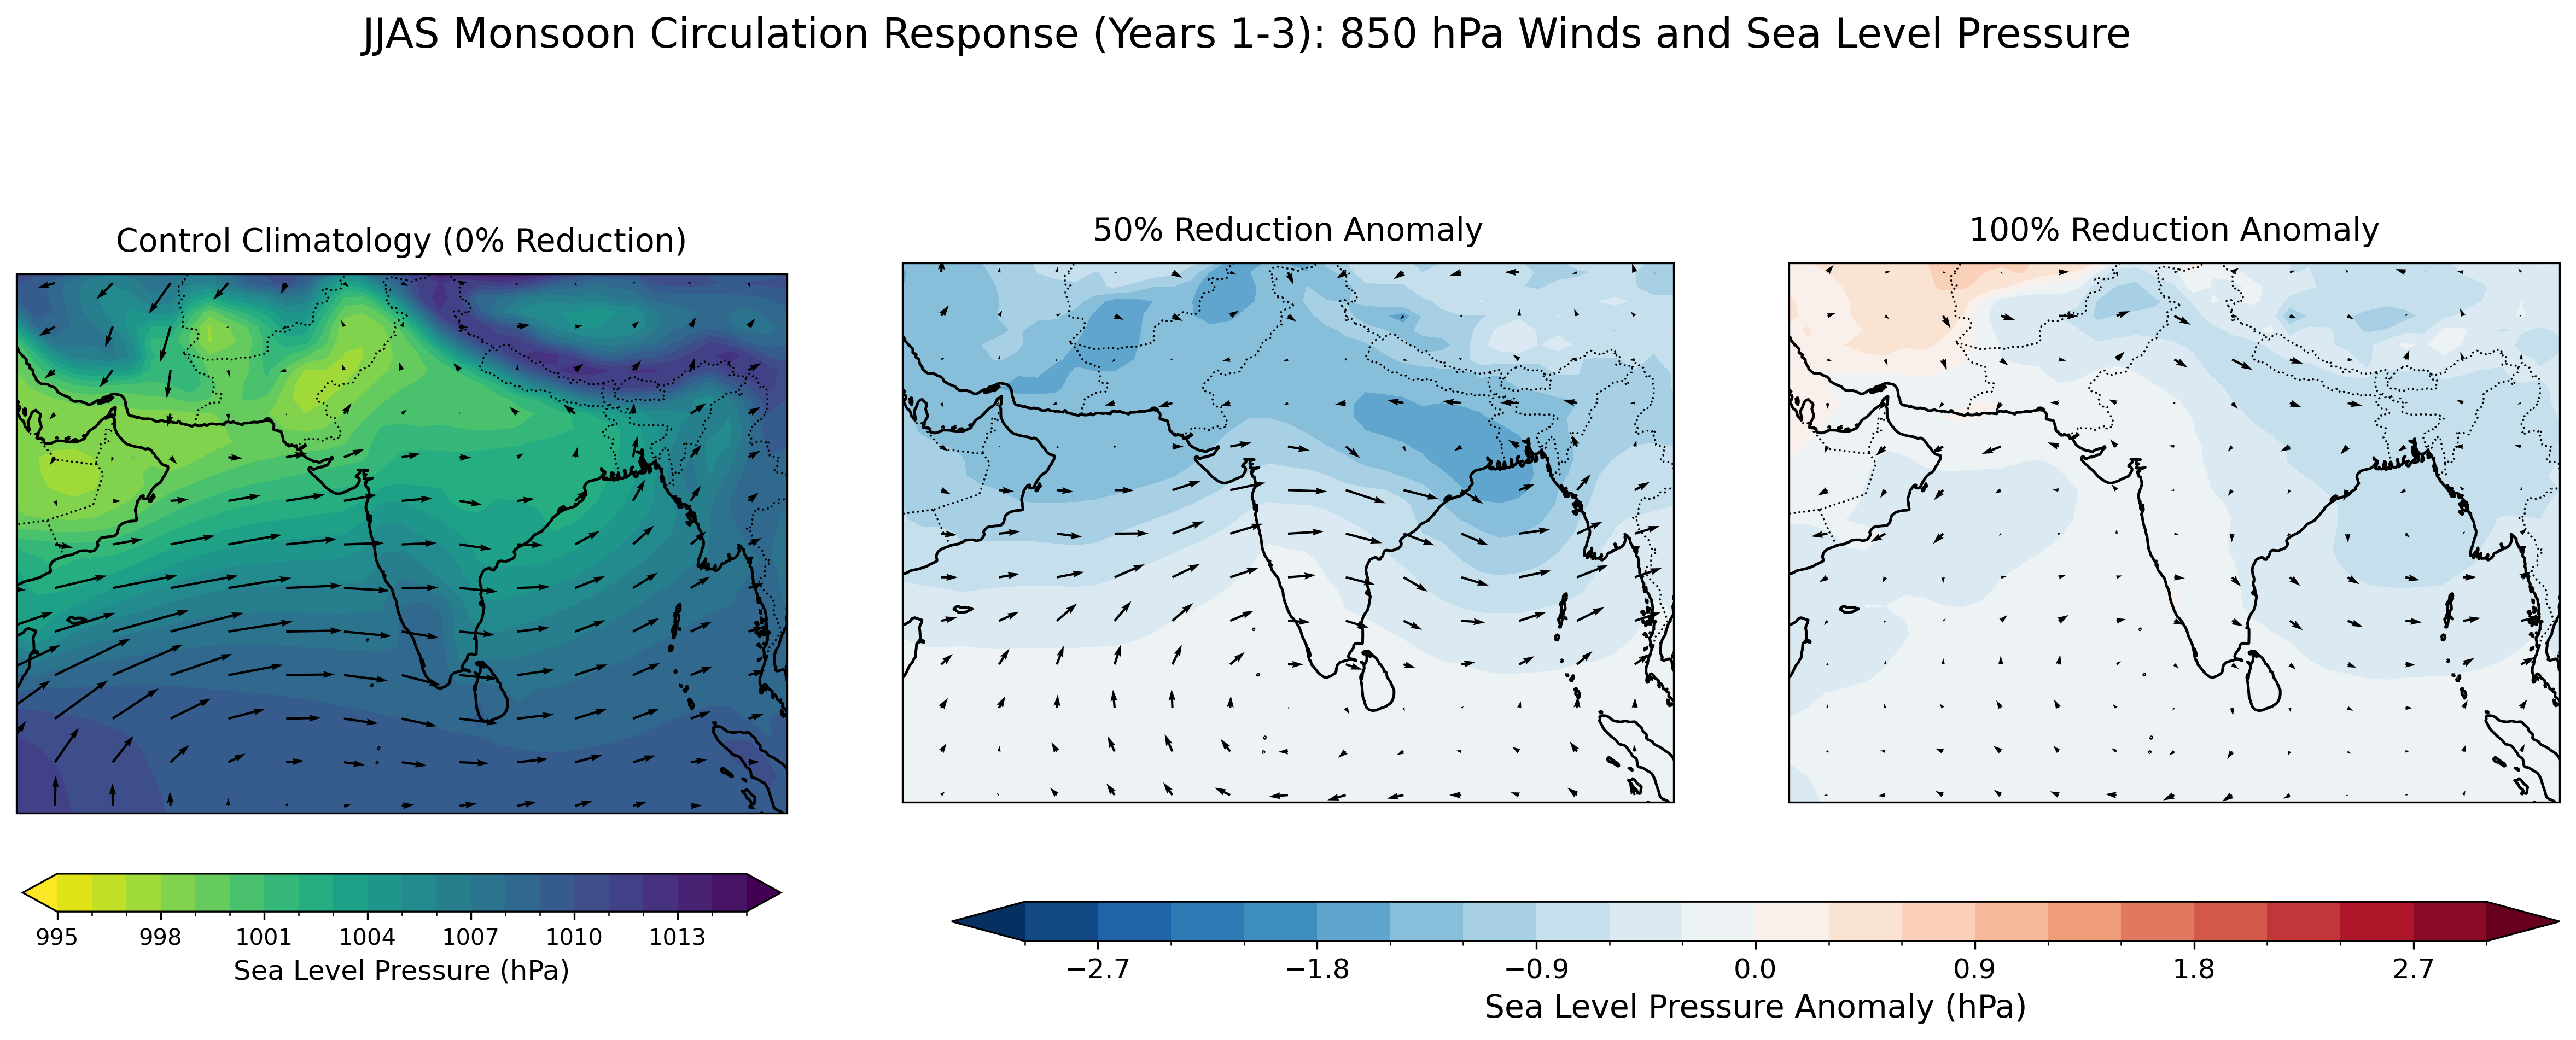
\includegraphics[width=\textwidth]{circulation.png}
    \caption{Wind and pressure in Indian region}
    \label{fig:wind_pressure_india}
\end{figure}
\indent We can see that reduction in aerosol concentration would lead to a stronger Indian summer monsoon(stronger winds). I am not sure why the anomaly is higher for the 50\% aerosol reduction case\\

\indent The following is the precipitation anomaly during Indian summer monsoon.\\
\begin{figure}[H]
    \centering
    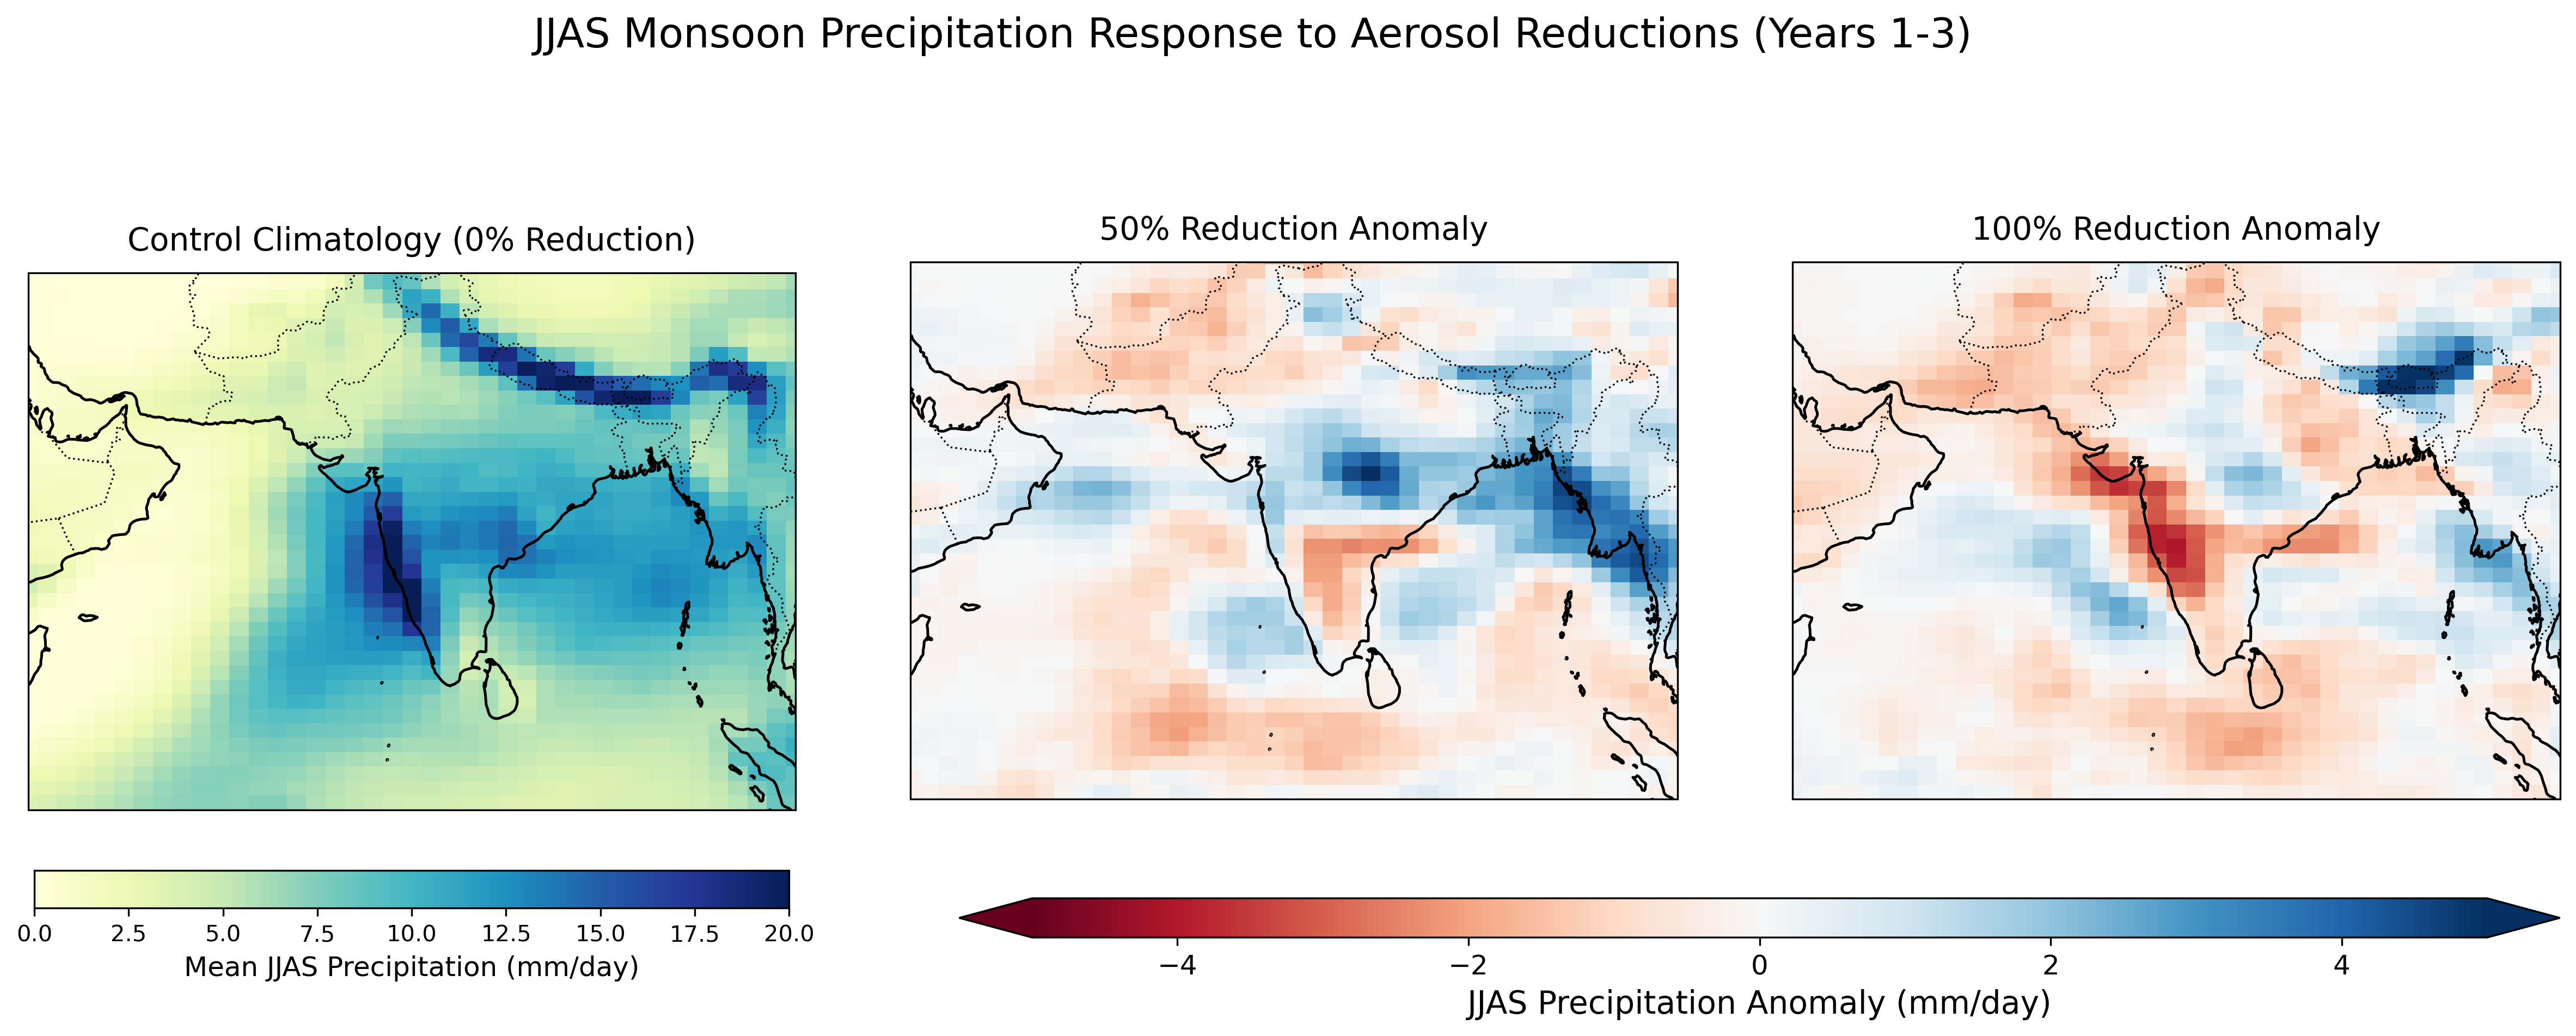
\includegraphics[width=\textwidth]{ind_monsoon_precip.png}
    \caption{Indian summer monsoon precipition}
    \label{fig:indian_monsoon}
\end{figure}

\section{Conclusion}

\indent From the study, we can conclude that reducing anthropogenic aerosol emission will lead to reudction in the number of cloud water droplets and will also result in a stronger Indian summer monsoon.\\
\indent Further study can be done for a longer time using a coupled ocean model for more accurate results.\\

\indent Python scripts and modified files are available at: \url{https://github.com/AgS-a/anthro-aerosol}\\ 

%\printbibliography

\end{document}
